Owing to imperfection of original photos or some irregular situations that the above algorithms do not handle, there might be blobs on the photos. We implement blob removal based on a feature in OpenCV libraries, \texttt{cv::SimpleBlobDetector}. Using the following function (need to include \texttt{features2d.hpp})
\begin{lstlisting}
  static Ptr<SimpleBlobDetector> cv::create(
    const SimpleBlobDetector::Params &parameters=SimpleBlobDetector::Params()
  )
\end{lstlisting}
simply convert RGB color to gray scale only, which may not detect the blobs completely; what's more, splitting RGB color into three channels and thresholding by each channel are not effective enough. Hence, we transform RGB color to \textbf{Lab color space} and threshold the image by \textbf{L} (lightness), \textbf{a} (green-red color component), and \textbf{b} (blue-yellow color component) channels separately, which may have better performance for blob detection, and then use the original \texttt{cv::SimpleBlobDetector} functions to detect the blobs.

This feature is realized by the following function in \texttt{src/util.cpp}
\begin{lstlisting}
  void blob_removal(const Mat& pic, Mat& result)
\end{lstlisting}
Since \texttt{cv::SimpleBlobDetector} provides many parameters for blob detection, such as blob size, circularity, inertia ratio, convexity, and for convenience, we create a panel for tuning these parameters (Fig. \ref{fig:blob-panel}). One of the advantages is that we can manually figure out the correctness of blob detection, and thus prevent the detection from some unwanted results if performing automatically. However, iterations is required for completeness since different blobs may have their own threshold values.

\begin{figure}[!ht]
  \centering
  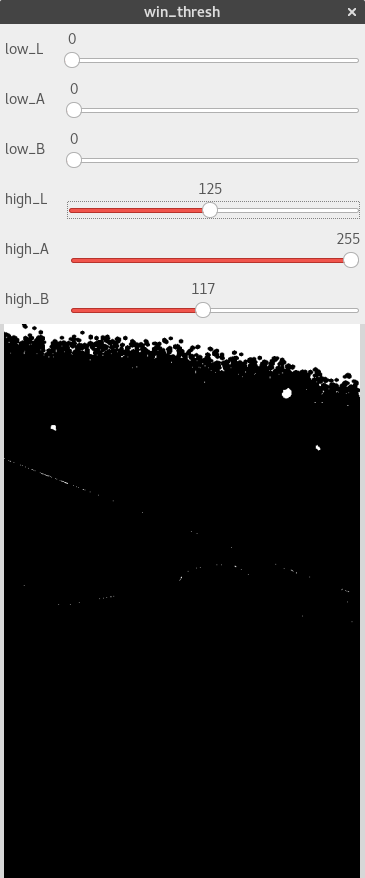
\includegraphics[height=16cm]{blob-panel1}
  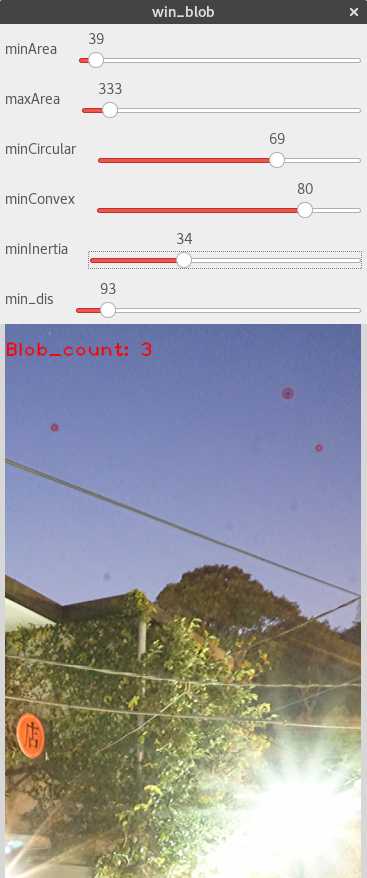
\includegraphics[height=16cm]{blob-panel2}
  \caption{Panel for blob removal}
  \label{fig:blob-panel}
\end{figure}

Once the blobs are detected, we approximately fill out these areas with the average colors nearby. For more details, one can refer to \texttt{src/util.hpp} and \texttt{src/util.cpp}. 